\section{Database}

As shown on the Figure \ref{fig:database} it can be appreciated that the database consists on 6 tables, each table has a different type of relationship from one another. Most of the relationships shown on the diagram are a one-to-many relationship, there is just one relationship many-to-many between Analyses and Vulnerabilities.

The tables have the following usage/meaning:

\begin{itemize}
    \item Users - stores the user's information.
    \item Analyses - stores each analysis made by a user.
    \item Vulnerabilities - stores the information of the 10 vulnerabilities that can be scanned, each vulnerability is unique so it cannot be repeated.
    \item Analysis-has-Vulnerabilities - it is a relationship between an analysis and all the vulnerabilities that have to be scanned for that specific analysis.
    \item Security-Flaws - stores the data of an specific flaw found on an specific analysis.
    \item Notifications - stores the information of the notifications shown on the site related to a user.
\end{itemize}

\begin{figure}[h!]
    \centering
    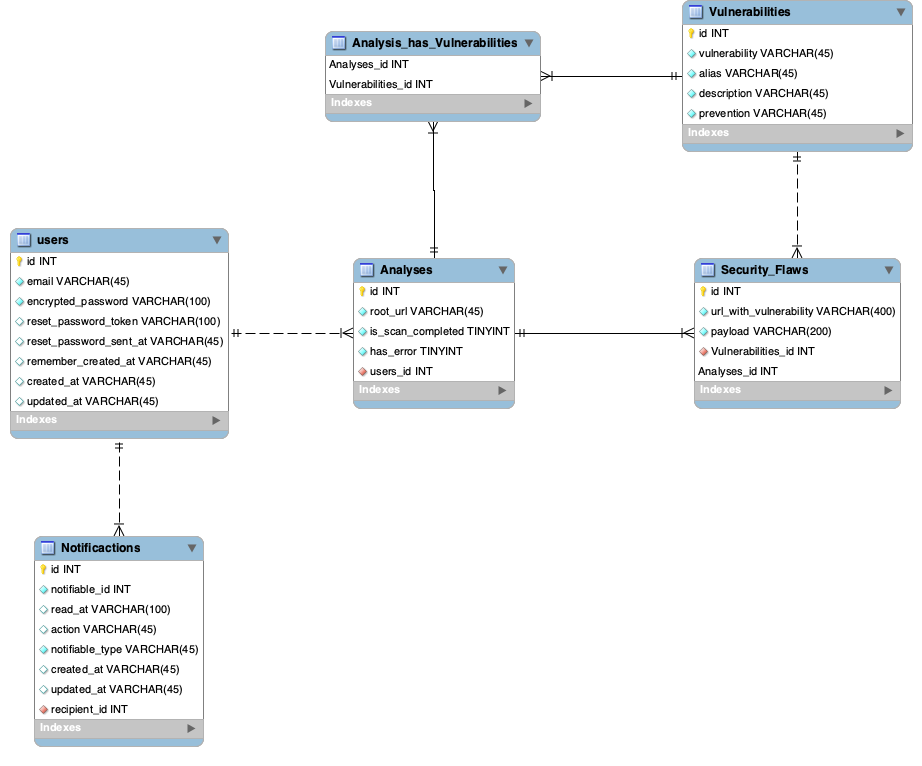
\includegraphics[width=13cm]{img/Databae.png}
    \caption{Relational database's model}
    \label{fig:database}
\end{figure}
